%% Beginning of file 'sample631.tex'
%%
%% Modified 2021 March
%%
%% This is a sample manuscript marked up using the
%% AASTeX v6.31 LaTeX 2e macros.
%%
%% AASTeX is now based on Alexey Vikhlinin's emulateapj.cls 
%% (Copyright 2000-2015).  See the classfile for details.

%% AASTeX requires revtex4-1.cls and other external packages such as
%% latexsym, graphicx, amssymb, longtable, and epsf.  Note that as of 
%% Oct 2020, APS now uses revtex4.2e for its journals but remember that 
%% AASTeX v6+ still uses v4.1. All of these external packages should 
%% already be present in the modern TeX distributions but not always.
%% For example, revtex4.1 seems to be missing in the linux version of
%% TexLive 2020. One should be able to get all packages from www.ctan.org.
%% In particular, revtex v4.1 can be found at 
%% https://www.ctan.org/pkg/revtex4-1.

%% The first piece of markup in an AASTeX v6.x document is the \documentclass
%% command. LaTeX will ignore any data that comes before this command. The 
%% documentclass can take an optional argument to modify the output style.
%% The command below calls the preprint style which will produce a tightly 
%% typeset, one-column, single-spaced document.  It is the default and thus
%% does not need to be explicitly stated.
%%
%% using aastex version 6.3
%\documentclass[linenumbers,preprint2]{aastex631}
\documentclass[twocolumn]{aastex631}

%% The default is a single spaced, 10 point font, single spaced article.
%% There are 5 other style options available via an optional argument. They
%% can be invoked like this:
%%
%% \documentclass[arguments]{aastex631}
%% 
%% where the layout options are:
%%
%%  twocolumn   : two text columns, 10 point font, single spaced article.
%%                This is the most compact and represent the final published
%%                derived PDF copy of the accepted manuscript from the publisher
%%  manuscript  : one text column, 12 point font, double spaced article.
%%  preprint    : one text column, 12 point font, single spaced article.  
%%  preprint2   : two text columns, 12 point font, single spaced article.
%%  modern      : a stylish, single text column, 12 point font, article with
%% 		  wider left and right margins. This uses the Daniel
%% 		  Foreman-Mackey and David Hogg design.
%%  RNAAS       : Supresses an abstract. Originally for RNAAS manuscripts 
%%                but now that abstracts are required this is obsolete for
%%                AAS Journals. Authors might need it for other reasons. DO NOT
%%                use \begin{abstract} and \end{abstract} with this style.
%%
%% Note that you can submit to the AAS Journals in any of these 6 styles.
%%
%% There are other optional arguments one can invoke to allow other stylistic
%% actions. The available options are:
%%
%%   astrosymb    : Loads Astrosymb font and define \astrocommands. 
%%   tighten      : Makes baselineskip slightly smaller, only works with 
%%                  the twocolumn substyle.
%%   times        : uses times font instead of the default
%%   linenumbers  : turn on lineno package.
%%   trackchanges : required to see the revision mark up and print its output
%%   longauthor   : Do not use the more compressed footnote style (default) for 
%%                  the author/collaboration/affiliations. Instead print all
%%                  affiliation information after each name. Creates a much 
%%                  longer author list but may be desirable for short 
%%                  author papers.
%% twocolappendix : make 2 column appendix.
%%   anonymous    : Do not show the authors, affiliations and acknowledgments 
%%                  for dual anonymous review.
%%
%% these can be used in any combination, e.g.
%%
%% \documentclass[twocolumn,linenumbers,trackchanges]{aastex631}
%%
%% AASTeX v6.* now includes \hyperref support. While we have built in specific
%% defaults into the classfile you can manually override them with the
%% \hypersetup command. For example,
%%
%% \hypersetup{linkcolor=red,citecolor=green,filecolor=cyan,urlcolor=magenta}
%%
%% will change the color of the internal links to red, the links to the
%% bibliography to green, the file links to cyan, and the external links to
%% magenta. Additional information on \hyperref options can be found here:
%% https://www.tug.org/applications/hyperref/manual.html#x1-40003
%%
%% Note that in v6.3 "bookmarks" has been changed to "true" in hyperref
%% to improve the accessibility of the compiled pdf file.
%%
%% If you want to create your own macros, you can do so
%% using \newcommand. Your macros should appear before
%% the \begin{document} command.
%%
\usepackage{xspace}
\usepackage{amsmath}
\usepackage{longtable}


\newcommand{\vdag}{(v)^\dagger}
\newcommand\aastex{AAS\TeX}
\newcommand\latex{La\TeX}

\newcommand{\rhk}{$R'_\mathrm{HK}$\xspace}
\newcommand{\shk}{$S_\mathrm{HK}$\xspace}
\newcommand{\caiihk}{Ca II H\&K \xspace}

\newcommand{\rocrit}{$\mathrm{Ro_{crit}}$\xspace}

\newcommand{\kms}{km~s$^{-1}$}
\newcommand{\ms}{m~s$^{-1}$}
\newcommand{\gcc}{g~cm$^{-3}$}
\newcommand{\masyr}{mas~yr$^{-1}$}
\newcommand{\err}{\textit{$\pm$}}

\newcommand{\Mstar}{\ensuremath{M_{\star}}\xspace}
\newcommand{\Rstar}{\ensuremath{R_{\star}}\xspace} 
\newcommand{\Lstar}{\ensuremath{L_{\star}}\xspace} 
\newcommand{\teff}{\ensuremath{T_{\mathrm{eff}}}\xspace}  
\newcommand{\logg}{\ensuremath{\log g}\xspace} 
\newcommand{\feh}{[Fe/H]\xspace}
\newcommand{\vsini}{\ensuremath{v \sin i}\xspace} 
\newcommand{\prot}{\ensuremath{P_\mathrm{rot}}\xspace}
\newcommand{\rvar}{\ensuremath{R_\mathrm{var}}\xspace}
\newcommand{\vtan}{\ensuremath{v_\mathrm{tan}}\xspace}
\newcommand{\vb}{\ensuremath{v_\mathrm{b}}\xspace}

\newcommand{\mearth}{$M_\oplus$\xspace}
\newcommand{\rearth}{$R_\oplus$\xspace}

\newcommand{\msun}{$M_\odot$\xspace}
\newcommand{\rsun}{$R_\odot$\xspace}
\newcommand{\lsun}{$L_\odot$\xspace}
\newcommand{\rhosun}{$\rho_\odot$\xspace}
\newcommand{\mstar}{$M_*$\xspace}
\newcommand{\rstar}{$R_*$\xspace}
\newcommand{\lstar}{$L_*$\xspace}
\newcommand{\rhostar}{$\rho_*$\xspace}


\newcommand{\logage}{$\text{log(age)}$\xspace}
\newcommand{\rp}{$R_P$\xspace}
\newcommand{\rprstar}{$R_P/R_\star$\xspace}

\newcommand{\logrp}{$\log_{10}(R_P/R_\oplus)$\xspace}
\newcommand{\deltaage}{$\Delta \log_{10}(\mathrm{age~yr}^{-1})$\xspace}
\newcommand{\deltamstar}{$\Delta M_*$\xspace}
\newcommand{\deltateff}{$\Delta T_\mathrm{eff}$\xspace}

\newcommand{\mjup}{$M_\mathrm{Jup}$\xspace}
\newcommand{\galex}{\textit{GALEX}\xspace}
\newcommand{\gaia}{\textit{Gaia}\xspace}
\newcommand{\kepler}{\textit{Kepler}\xspace}
\newcommand{\spitzer}{\textit{Spitzer}}
\newcommand{\hipparcos}{\textit{Hipparcos}}
\newcommand{\ktwo}{\textit{K2}\xspace}
\newcommand{\tess}{\textit{TESS}\xspace}
\newcommand{\emcee}{\texttt{emcee}\xspace}
\newcommand{\stardate}{\texttt{stardate}\xspace}
\newcommand{\python}{\textsc{python}\xspace}

\newcommand{\ymg}{[Y/Mg]\xspace}
\newcommand{\yal}{[Y/Al]\xspace}
\newcommand{\alphafe}{[$\alpha$/Fe]\xspace}
\newcommand{\dexgyr}{dex~Gyr$^{-1}$\xspace}


%% Reintroduced the \received and \accepted commands from AASTeX v5.2
%\received{March 1, 2021}
%\revised{April 1, 2021}
%\accepted{\today}

%% Command to document which AAS Journal the manuscript was submitted to.
%% Adds "Submitted to " the argument.
%\submitjournal{PSJ}

%% For manuscript that include authors in collaborations, AASTeX v6.31
%% builds on the \collaboration command to allow greater freedom to 
%% keep the traditional author+affiliation information but only show
%% subsets. The \collaboration command now must appear AFTER the group
%% of authors in the collaboration and it takes TWO arguments. The last
%% is still the collaboration identifier. The text given in this
%% argument is what will be shown in the manuscript. The first argument
%% is the number of author above the \collaboration command to show with
%% the collaboration text. If there are authors that are not part of any
%% collaboration the \nocollaboration command is used. This command takes
%% one argument which is also the number of authors above to show. A
%% dashed line is shown to indicate no collaboration. This example manuscript
%% shows how these commands work to display specific set of authors 
%% on the front page.
%%
%% For manuscript without any need to use \collaboration the 
%% \AuthorCollaborationLimit command from v6.2 can still be used to 
%% show a subset of authors.
%
%\AuthorCollaborationLimit=2
%
%% will only show Schwarz & Muench on the front page of the manuscript
%% (assuming the \collaboration and \nocollaboration commands are
%% commented out).
%%
%% Note that all of the author will be shown in the published article.
%% This feature is meant to be used prior to acceptance to make the
%% front end of a long author article more manageable. Please do not use
%% this functionality for manuscripts with less than 20 authors. Conversely,
%% please do use this when the number of authors exceeds 40.
%%
%% Use \allauthors at the manuscript end to show the full author list.
%% This command should only be used with \AuthorCollaborationLimit is used.

%% The following command can be used to set the latex table counters.  It
%% is needed in this document because it uses a mix of latex tabular and
%% AASTeX deluxetables.  In general it should not be needed.
%\setcounter{table}{1}

%%%%%%%%%%%%%%%%%%%%%%%%%%%%%%%%%%%%%%%%%%%%%%%%%%%%%%%%%%%%%%%%%%%%%%%%%%%%%%%%
%%
%% The following section outlines numerous optional output that
%% can be displayed in the front matter or as running meta-data.
%%
%% If you wish, you may supply running head information, although
%% this information may be modified by the editorial offices.
\shorttitle{The Rossby Ridge}
\shortauthors{David et al.}
%%
%% You can add a light gray and diagonal water-mark to the first page 
%% with this command:
%% \watermark{text}
%% where "text", e.g. DRAFT, is the text to appear.  If the text is 
%% long you can control the water-mark size with:
%% \setwatermarkfontsize{dimension}
%% where dimension is any recognized LaTeX dimension, e.g. pt, in, etc.
%%
%%%%%%%%%%%%%%%%%%%%%%%%%%%%%%%%%%%%%%%%%%%%%%%%%%%%%%%%%%%%%%%%%%%%%%%%%%%%%%%%
\graphicspath{{./}{figures/}}
%% This is the end of the preamble.  Indicate the beginning of the
%% manuscript itself with \begin{document}.

\begin{document}

% \title{The Rossby Ridge: a Pile-up of Rapidly Rotating Main-Sequence Stars with a Broad Range of Ages}
\title{A Pile-up of Rapidly Rotating Main-Sequence Stars with a Broad Range of Ages: \\Further Evidence for Weakened Magnetic Braking}

%\\or\\Weakened Magnetic Braking Supported by Rotation Rates of Kepler Exoplanet Hosts}

% Ridge
% Edge
% Ledge
% Cornice

\correspondingauthor{Trevor J. David}
\email{tdavid@flatironinstitute.org}

\author[0000-0001-6534-6246]{Trevor J.\ David}
\affil{Center for Computational Astrophysics, Flatiron Institute, New York, NY 10010, USA}
\affil{Department of Astrophysics, American Museum of Natural History, Central Park West at 79th Street, New York, NY 10024, USA}

\author[0000-0003-4540-5661]{Ruth Angus}
\affil{Department of Astrophysics, American Museum of Natural History, Central Park West at 79th Street, New York, NY 10024, USA}
\affil{Center for Computational Astrophysics, Flatiron Institute, New York, NY 10010, USA}
\affil{Department of Astronomy, Columbia University, 550 West 120th Street, New York, NY, USA}

\author[0000-0002-2792-134X]{Jason L.~Curtis}
\affil{Department of Astronomy, Columbia University, 550 West 120th Street, New York, NY, USA}

\author[0000-0002-4284-8638]{Jennifer van Saders}
\affil{Institute for Astronomy, University of Hawai’i, Honolulu, HI, USA}

\author[0000-0002-3011-4784]{Gabriella Contardo}
\affil{Center for Computational Astrophysics, Flatiron Institute, New York, NY 10010, USA}

\author{Other authors TBD}

%Gaby Contardo
%Lucy Lu
%Joel Zinn
%Adrian Price-Whelan


\begin{abstract}
We combine stellar surface rotation periods determined from NASA's Kepler mission with spectroscopic parameters derived from the California-Kepler Survey and LAMOST--Kepler survey to demonstrate the existence of a long-period pile-up in the effective temperature--rotation period distribution of main-sequence stars with temperatures exceeding 5800~K. Stars in the pile-up are found to have a wide range of ages ($\sim$2--6~Gyr), meaning that, along the ridge, rotation period is strongly predictive of a star's surface temperature but only weakly predictive of its age. In the effective temperature range of 5000--6250~K the long-period pile-up is well-described by a single-parameter model of constant Rossby number, with a critical value of $\mathrm{Ro_{crit}} \sim$\textbf{XYZ}. The long-period pile-up was previously predicted by \citet{vanSaders2019} as a consequence of weakened magnetic braking, in which stellar spin-down stalls once stars reach a critical Rossby number. These results imply that surface rotation periods have limited predictive power for the age determination of F- and early G-type stars older than $\sim$1--2~Gyr. \textbf{We additionally detect a secondary pile-up associated with the short-period edge of the rotation period distribution.}
\end{abstract}

%% Keywords should appear after the \end{abstract} command. 
%% The AAS Journals now uses Unified Astronomy Thesaurus concepts:
%% https://astrothesaurus.org
%% You will be asked to selected these concepts during the submission process
%% but this old "keyword" functionality is maintained in case authors want
%% to include these concepts in their preprints.
\keywords{Stellar rotation (1629) --- Stellar evolution (1599) --- Stellar magnetic fields (1610) --- F dwarf stars(516)}

%% From the front matter, we move on to the body of the paper.
%% Sections are demarcated by \section and \subsection, respectively.
%% Observe the use of the LaTeX \label
%% command after the \subsection to give a symbolic KEY to the
%% subsection for cross-referencing in a \ref command.
%% You can use LaTeX's \ref and \label commands to keep track of
%% cross-references to sections, equations, tables, and figures.
%% That way, if you change the order of any elements, LaTeX will
%% automatically renumber them.
%%
%% We recommend that authors also use the natbib \citep
%% and \citet commands to identify citations.  The citations are
%% tied to the reference list via symbolic KEYs. The KEY corresponds
%% to the KEY in the \bibitem in the reference list below. 

\section{Introduction} \label{sec:intro}
Solar-type and low-mass stars ($M\lesssim1.3$~\msun) lose mass and angular momentum through magnetized winds \citep{Parker1958, WeberDavis1967, Mestel1968, Kawaler1988}. Consequently, stellar rotation rates are observed to decline with age. \citet{Skumanich1972} presented the first attempt to calibrate this age-rotation relationship using the rotation periods of Sun-like stars in open clusters with independently determined ages, finding a $P_\mathrm{rot} \propto t^{1/2}$ scaling, where $t$ is stellar age. In the intervening decades, observational determinations of stellar rotation periods among open cluster members revealed how stellar spin rates evolve in more detail, leading to the calibration of the so-called gyrochronology method \citep{Barnes2003, Barnes2007, Barnes2010, MamajekHillenbrand2008, Meibom2009}.

The arrival of continuous, high-precision, long-baseline photometry from NASA's Kepler space telescope \citep{Borucki2010} provided a watershed moment for stellar rotation studies, yielding period detections for tens of thousands of stars \citep[e.g.][]{Reinhold2013, McQuillan2014, Santos2021} and allowing for gyrochronology to be extended to older ages \citep[e.g.][]{Meibom2011, Meibom2015}. NASA's subsequent K2 \citep{Howell2014} and TESS \citep{Ricker2015} missions propelled the field of stellar rotation further still, providing an exquisitely detailed picture of how spin rates evolve for stars with a broad range of masses and ages in stellar associations \citep[e.g.][]{Douglas2016, Douglas2017, Douglas2019, Rebull2016, Rebull2017, Rebull2018, Rebull2020, Curtis2019a, Curtis2019b, Curtis2020}. New and evermore precise data is becoming available at a rate that is outpacing efforts to re-calibrate gyrochronology, which is necessary to capture the complex relationship between a star's spin and its age. 

%Nevertheless, it is by now clear that the simple $t^{1/2}$ scaling of rotation rates with age breaks down in certain regimes of stellar mass and age. Efforts to calibrate gyrochronology relations using Kepler asteroseismic targets revealed tension with relations calibrated to open clusters and found that rotation periods could not be described by a single power-law relation with age \citep{Angus2015}. More recently, low-mass stars were shown to experience a temporary epoch of stalled spin-down which is not accounted for by standard gyrochronology models \citep{Curtis2019a}. \citet{Spada2020} and \citet{Curtis2020} proposed that this epoch of apparent stalling may arise from rotational coupling of the core and envelope, in which redistribution of angular momentum from the interior to the surface temporarily offsets the effects of magnetic braking. Regardless of the true mechanism, rotation periods in this part of parameter space have diminished utility in predicting stellar ages. 

For example, efforts to calibrate gyrochronology relations using Kepler asteroseismic targets revealed tension with relations calibrated to open clusters and found that rotation periods could not be described by a single power-law relation with age \citep{Angus2015}. This tension, at least in part, is due to the fact that standard gyrochronology models are unable to account for the anomalously rapid rotation rates of stars older than the Sun, leading to the suggestion that stars with masses $\gtrsim$~1\msun experience a phase of weakened magnetic braking \citep[WMB,][]{vanSaders2016}. Forward modeling simulations of the observed Kepler rotation period distribution also provided support for the WMB hypothesis over standard spin-down models, in that WMB models are better able to match the observed long-period edge \citep{vanSaders2019}. Those authors also predicted a pile-up of stars along the long-period edge, which they hypothesized could not be seen in the \citet{McQuillan2014} sample due to large errors on \teff in the Kepler Input Catalog \citep[KIC,][]{Brown2011}. While \citet{vanSaders2019} favored the WMB hypothesis to explain observations, those authors were also careful to point out that a long-period edge can be caused by detection biases, as stars with longer rotation periods (and larger Rossby numbers) have smaller amplitude variations which pose more difficulty to period-detection algorithms. 

More recently, \citet{Hall2021} used the asteroseismic rotation rates of Kepler dwarfs, with a different selection bias from the \citet{vanSaders2019} study and the present work, to argue support for the WMB model. While the physics responsible for the weakened magnetic braking of solar-type stars is unknown, one hypothesis is that the declining efficiency of wind-driven angular momentum loss is connected to the magnetic field complexity, which varies with Rossby number \citep[e.g.][]{Reville2015, vanSaders2016, Garraffo2016, Metcalfe2016, Metcalfe2019}.  

%Similar to the apparent stalling of low-mass stars mentioned above, 

%If this is the case, a time-dependent (or, more accurately, Rossby-dependent) magnetic field morphology might explain both the anomalously rapid rotation of old field stars and the existence of a detection edge, as the amplitude of variability should also be connected to the field morphology.

%period-detection algorithms are less efficient for stars with (i) smaller amplitude variations, and (ii) quasi-periodic or stochastic variations. The 
%number, size, contrast, and relative orientations of spots on the surface of stars

Here we examine the rotation period distribution of main-sequence stars observed by Kepler, leveraging the recent release of precise spectroscopic parameters from large-scale surveys, to demonstrate the existence of a long-period pile-up for F- and early G-type stars. \textbf{In this work we refer to this feature as the long-period pile-up, the Rossby ridge, or simply the ridge.} We argue that several aspects of this pile-up feature are consistent with expectations from the WMB model. We discuss our sample in \S\ref{sec:sample}, describe the steps of our analysis in \S\ref{sec:analysis}, and present our conclusions in \S\ref{sec:conclusions}.

\section{Sample Selection} \label{sec:sample}
Below, we describe the samples utilized in this work. All stars characterized here were targets of NASA's Kepler mission \citep{Borucki2010} and have published rotation periods derived from the Kepler data.

%We consider two samples in this work. The first sample is derived from the CKS sample, which itself is a subset of Kepler exoplanet candidate host stars that were spectroscopically characterized in a homogeneous manner. The second sample arises from a cross-match of the Kepler field with the LAMOST spectroscopic survey \textbf{(citation)}.

\begin{figure*}
    \centering
    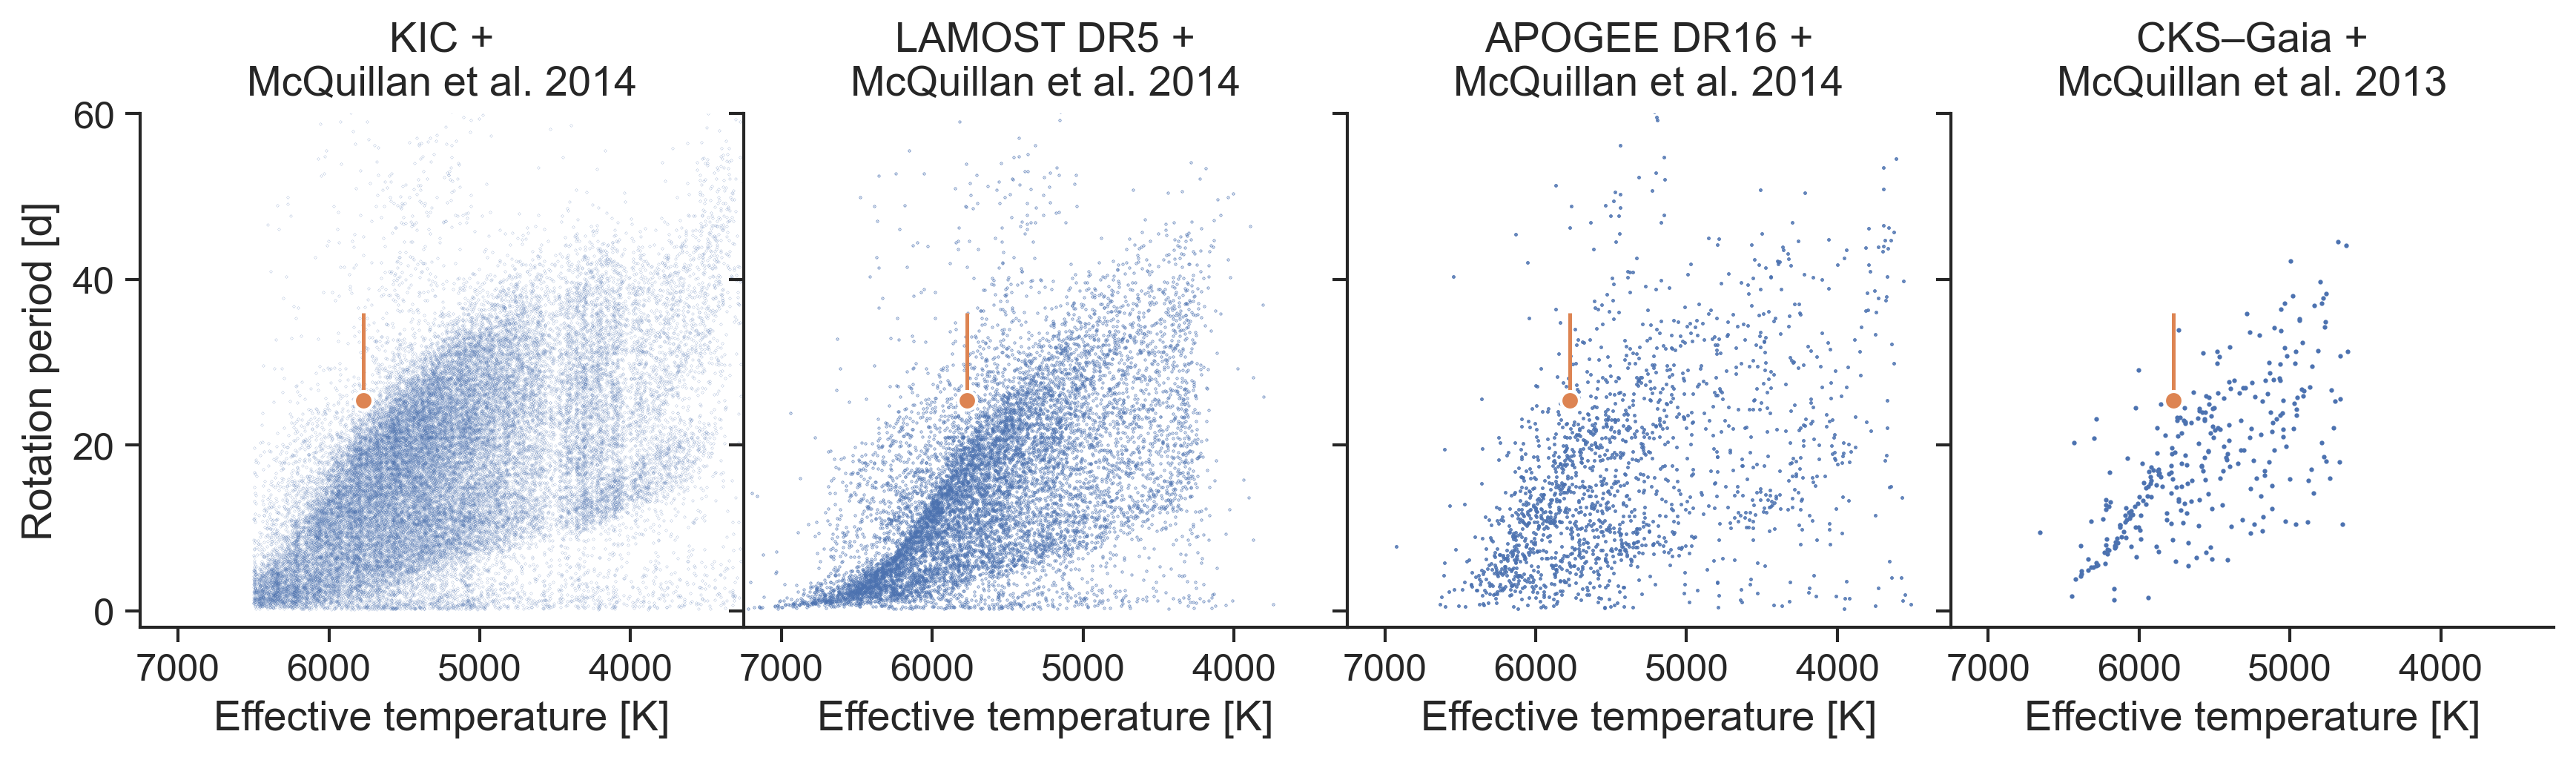
\includegraphics[width=\textwidth]{surveys.pdf}
    \caption{The \teff-\prot plane using rotation periods from \citet{McQuillan2014} or, in the case of the CKS sample, \citet{McQuillan2013}, with \teff originating from the source denoted at top. The \citet{McQuillan2014} \teff values originate from the Kepler Input Catalog \citep[KIC,][]{Brown2011} or \citet{Dressing2013} for low-mass stars. The orange point in each panel indicates the Sun's equatorial rotation period, with the errorbar capturing the range of periods measured from the differentially rotating surface.}
    \label{fig:surveys}
\end{figure*}

\subsection{California--Kepler Survey} \label{sec:cks}
The CKS project gathered high-resolution spectroscopy for 1305 Kepler planet host stars \citep{Petigura2017}. CKS spectra were acquired with the Keck/HIRES spectrograph \citep{Vogt1994} and spectroscopic parameters were determined by averaging parameters from the SpecMatch pipeline \citep{Petigura2015} and SME@XSEDE, a Python implementation of the Spectroscopy Made Easy pipeline \citep{Valenti1996}. The internal errors on \teff from the CKS catalog are 60~K.

We compiled rotation periods for these stars from a variety of literature sources including \citet{McQuillan2013, Mazeh2015} and \citet{Angus2018}. For each star in the sample we then visually inspected the Kepler light curve folded on all available literature periods, as well as the first harmonics and sub-harmonics of those periods, and recorded our preferred period along with a reliability flag. Our procedure is explained in detail in \S2.1 of \citet{David2021}, and rotation period vetting sheets for each Kepler Object of Interest (KOI) are publicly available through Zenodo.\footnote{\url{http://10.0.20.161/zenodo.4645437}} We note that the vast majority of stars in the CKS sample host small planets ($R_P < 4$~\rearth) and as such it is not expected that the host stars have experienced tidal spin-up from the planets.

In addition to the original CKS catalog, we also cross-matched our sample with the catalogs of \citet{Brewer2018} and \citet{Martinez2019}, both of which presented spectroscopic parameters for CKS stars based on independent analysis of the same spectra. The \citet{Brewer2018} study, referred to here as SPOCS, also published elemental abundances and ages from isochrone fitting for the CKS sample.

\iffalse
\begin{figure*}
    \centering
    \includegraphics[width=\linewidth]{ridge.pdf}
    \caption{The \teff-\prot plane for the CKS sample. Point colors are scaled to the CKS ages determined from isochrone fitting. The source of \prot is denoted above each panel, where \citet{David2021} is a compilation of vetted periods, rather than a source of original measurements. The black trapezoid indicates the approximate area of the ridge. The grey curves indicate empirical cluster sequences from \citet{Curtis2020}, corresponding to ages of $\sim$2.7, 1, 0.67, and 0.12~Gyr from top to bottom.}
    \label{fig:ridge}
\end{figure*}
\fi 

%Points on contours
%Different color for 
%, pixel 

\subsection{LAMOST--Kepler} \label{sec:lamost}
The LAMOST--Kepler project derived homogeneous spectroscopic parameters from low-resolution ($R\sim$~1800) LAMOST DR5 spectra for approximately 40\% of the Kepler field \citep{Zong2018, Xiang2019}. We cross-matched the LAMOST--Kepler stellar parameter catalog of \citet{Xiang2019} with the \citet{McQuillan2014} rotation period catalog, which published rotation periods for $>$34000 Kepler targets. The \citet{Xiang2019} catalog derived stellar parameters using the DD-Payne pipeline, which builds on the method of \citet{Ting2017b} by incorporating elements of the Cannon \citep{Ness2015}. 

We matched 10844 LAMOST targets to 10650 unique Kepler IDs. For the Kepler sources with duplicate cross-matched LAMOST sources we kept the source with a brighter Gaia DR2 $G$ magnitude. We additionally selected sources with 3000~K$< \teff <$~8000~K, 3$<$~\logg~$<$5 dex, and -2~$<$[Fe/H]$<$~2 dex. The final sample contains 10516 unique targets with well-determined \prot and \teff (having a median error of 24~K). There is negligible overlap (only 3 stars) between our LAMOST--Kepler samples and the CKS samples since the \citet{McQuillan2014} did not publish rotation periods for KOIs, which were the targets of the CKS project. 

%\textbf{Jason: can you provide any relevant background info and describe the rationale behind the cuts you made to ensure the cross-match was relatively good?}

\textbf{We additionally cross-matched the LAMOST--Kepler catalog with the CKS catalog...Note, LAMOST catalog contains duplicates from multiple visits. Describe how we handle these.}

\subsection{APOGEE--Kepler}
The Apache Point Observatory Galactic Evolution Experiment \citep[APOGEE,][]{Majewski2017} is a large-scale, high-resolution ($R \sim 22500$) stellar spectroscopic survey conducted at $H$-band as part of the Sloan Digital Sky Survey \citep[SDSS-IV][]{Blanton2017}. The spectroscopic analysis pipeline for SDSS DR16 is described in \citet{Jonsson2020}. We used Gaia DR2 source IDs \citep{Gaia2016, Gaia2018} to cross-match Megan Bedell's Gaia--Kepler catalog\footnote{\url{https://gaia-kepler.fun/}} with the APOGEE DR16 catalog \citep{Ahumada2020}. Kepler IDs were then used to cross-match this table with the \citet{McQuillan2014} catalog. While the current overlap between Kepler targets and APOGEE is small compared to the LAMOST catalog, APOGEE DR17 will contain more dwarf stars and provide a better resource for studies such as ours. The focus of this work are overdensities in the \teff--\prot plane, and as these appear to be less prominent when using  APOGEE DR16 temperatures (Figure~\ref{fig:surveys}) we conclude that LAMOST and CKS provide more accurate estimates of \teff and do not analyze the APOGEE sample further. 

\subsection{The Sun}
To place the Sun in the context of the long-period pile-up, we use up-to-date estimates of the Sun's effective temperature, rotation period, and age. Following the IAU 2015 Resolution B3 \citep{Mamajek2015}, we take the nominal effective temperature of the Sun to be $\mathcal{T}^\mathrm{N}_\mathrm{eff,\odot} = 5772$~K. For the solar rotation period we adopt the equatorial rotation period of $P_\mathrm{eq,\odot}~\approx~25$~d with an upper error that encompasses the period of $\approx$~36~d measured near the poles from differential rotation studies \citep[][and references therein]{Thompson2003}.  The age of the Sun is assumed to be 4.567~Gyr from Pb-Pb dating of calcium-aluminum inclusions and chondrules recovered from primitive meteorites \citep{Bahcall1995}.

%\prot = 26.09~d, with minimum and maximum periods of $P_\mathrm{min}=24.5$ and $P_\mathrm{max}=28.5$, from \citet{Donahue1996}. Measurements of differential rotation on the solar surface have found an equatorial period of approximately 25 days, increasing to about 36 days at the poles \citep[][and references therein]{Thompson2003}.

%\textbf{Measurements of differential rotation on the solar surface have found (SOHO/MDI results and possibly GONG...see e.g. Ulrich 1988)...}  


\section{Analysis}
\label{sec:analysis}

\subsection{Initial observations}
A pile-up of stars along the long-period edge for stars with \teff~$>5800$~K was first noted when examining the \teff-\prot plane for the CKS sample, using the CKS \teff values and the vetted rotation period compilation from \citet{David2021}. Sourcing rotation periods from \citet{McQuillan2013, Mazeh2015} and \citet{Angus2018} revealed that this pile-up is still apparent when adopting periods uniformly from a single catalog (Figure~\ref{fig:ridge}). 

The location of the pile-up approximately corresponds with an empirical hybrid cluster sequence derived by \citet{Curtis2020} from members of the NGC~6819 (age~$\sim$~2.5~Gyr) and Ruprecht~147 (age~$\sim$~2.7~Gyr) open clusters (Figure~\ref{fig:ridge}). As we show in \S\ref{subsec:ages}, stars along the long-period edge have a range of ages. Therefore, the observation that the edge approximately corresponds with the $\sim$2.5--2.7~Gyr cluster sequence implies that stars with \teff$\lesssim 5800~K$ have already piled up onto the edge by or before this timescale. Similarly, the edge is well-separated from the empirical $\sim$1~Gyr cluster sequence based on rotation rates in the NGC~6811 cluster \citep{Curtis2020}, implying that it takes F-type stars $>1$~Gyr to converge onto the long-period edge. These observations are in accordance with predictions from the WMB model which suggest the pile-up forms on a timescale of 2--3~Gyr \citep{vanSaders2019}.

Interestingly, in both the CKS and LAMOST samples, there appears to be a change of slope along the ridge, with an inflection point corresponding closely to the Kraft break at $\approx$6250~K, the point at which convective envelopes become vanishingly thin \citep{Kraft1967}. %\textbf{What to make of this? We can fit a model to the period distribution to measure exactly where the break is and test its significance.}

In the CKS sample, there appears to be a clustering of stars above the ridge with \teff~$>6100$~K. This cluster of points has a similar slope in the \teff--\prot plane as the ridge, and does not reside on the harmonic of the ridge line as one might expect if the periods were erroneously determined. After inspecting the light curves of stars on the ridge and above the ridge in the temperature range 6100~K~$<$~ \teff~$<6300$~K we did not notice any obvious trends or differences between the two samples. The periods of the stars in the cluster above the ridge appear to be just as reliable as those on the ridge. Interestingly, a similar clustering of points is not observed in the LAMOST--Kepler sample and is less pronounced or absent when substituting the CKS temperatures with \teff from either \citet{Brewer2018} or \citet{Martinez2019}, two studies that independently derived spectroscopic parameters from the CKS spectra. 

\subsection{Constant Rossby model}
\label{subsec:rossby}
In the WMB model of \citet{vanSaders2016, vanSaders2019}, a star spins down until it reaches a critical Rossby number, at which point magnetic braking is stalled. Since Rossby number is highly sensitive to temperature through its dependence on the convective turnover timescale ($\mathrm{Ro} = P_\mathrm{rot}/\tau_\mathrm{cz}$, where $\tau_\mathrm{cz}$ is the convective turnover timescale), this critical threshold corresponds to different rotation periods for stars of different \teff, leading to a pile-up in the \teff-\prot plane. Using a small sample of Kepler targets with rotation periods determined from brightness modulations, \citet{vanSaders2016} proposed this threshold happens at a critical Rossby number of $\mathrm{Ro_{crit}} \sim \mathrm{Ro_\odot}$. From a sample of Kepler targets with asteroseismic rotation rates, \citet{Hall2021} found a similar critical Rossby number of $\mathrm{Ro_{crit}} = 1.97$.

We tested the hypothesis that the long-period pile-up observed in the LAMOST--Kepler sample is due to WMB by fitting constant Rossby models to the \prot boundary. For a given \teff, this model predicts \prot as: 

\begin{equation}
    \prot (\mathrm{Ro}, \teff) = \mathrm{Ro} \times \tau_\mathrm{cz}(\teff),
\end{equation}

where we used the equation for the convective turnover timescale (valid in the \teff range of 3300~K$\lesssim \teff \lesssim$~7000~K) presented in \citet{Gunn1998} and replicated in \citet{CranmerSaar2011}:

\begin{multline}
\tau_\mathrm{cz}(\teff) = 314.24\exp \left [ -\left (\frac{T_\mathrm{eff}}{1952.5 \mathrm{K}}  \right ) - \left (\frac{T_\mathrm{eff}}{6250 \mathrm{K}}  \right )^{18} \right ] \\+ 0.002.
\end{multline}

To obtain a reasonable description of the long-period edge we computed the 90th percentile of \prot values in overlapping \teff bins with centers located every 20~K between 4000~K and 7000~K and half-widths of 100~K. We found it was also necessary to omit stars with Ro~$>$~5/3 in this computation to match the long period edge. Since we observed a break in the 90th percentile \prot curve near \teff~=~4250~K, due to smaller sample sizes at low \teff, we restricted the analysis below to stars with \teff$>~4250$~K. To compute approximate uncertainties on the 90th percentile curve we performed 100 bootstrapped resamplings in each bin, leaving out 50\% of the data for each resampling. The 90th percentile curve and its uncertainty was then computed from the mean and standard deviation of the boostrapped values. We computed the 10th percentile curve and its uncertainty similarly, as an approximation to the lower boundary of the \teff-\prot plane. We show these curves in relation to the full LAMOST--Kepler sample and to constant Rossby models in Figure~\ref{fig:pctl}.

\iffalse
\begin{figure}
    \centering
    \includegraphics[width=\linewidth]{pctl-curves.pdf}
    \caption{At top, The LAMOST--Kepler sample and the 10th and 90th \prot percentiles, computed as described in \S\ref{subsec:rossby}. At bottom, the same curves are shown in relation to fiducial constant Rossby models.}
    \label{fig:pctl}
\end{figure}
\fi 


%We computed constant Rossby models across the range of \teff bins using the equation for the convective turnover timescale presented in \citet{Gunn1998} and replicated in \citet{CranmerSaar2011}. This equation is valid in the \teff range of 3300~K$\lesssim \teff \lesssim$~7000~K. %\textbf{Note: we can also try Landin 2010 and Barnes Kim 2010 formulas for convective turnover timescales.}

We performed an initial Levenberg-Marquardt non-linear least-squares fit of a constant Rossby model to the long-period edge with the \texttt{curve\_fit} function in the \texttt{scipy.optimize} class to optimize the following likelihood: 

\begin{multline}
    \ln{p} (y | T_\mathrm{eff}, \sigma, \mathrm{Ro}, f) =\\ -\frac{1}{2}\sum_n \left [ \frac{(y_n - P_\mathrm{rot}(\mathrm{Ro}, T_\mathrm{eff}))^2}{s_n^2}  + \ln{(2\pi s_n^2)} \right ],
\end{multline}

where

\begin{equation}
    s_n^2 = \sigma^2 + f^2 P_\mathrm{rot}(\mathrm{Ro}, T_\mathrm{eff})^2,
\end{equation}

and $y_n$ is the value of a \prot percentile curve in the $n$th \teff bin. This is a Gaussian likelihood where the variance is underestimated by some fraction, $f$. We performed Markov chain Monte Carlo sampling (MCMC) of this likelihood with the \texttt{emcee} package \citep{emcee2013, emcee2019} to estimate the mean and uncertainty of the critical Rossby number that best matches the long-period edge in the range of 5000~K$\lesssim \teff \lesssim$~6250~K. We instantiated 32 walkers around the least-squares solution and sampled for $10^5$ steps, adopting uniform priors on Ro and $f$ with ranges of (0.1,10) and (0,10), respectively. Convergence was assessed by ensuring the chain length was at least 100 times longer than the chain autocorrelation lengths for each parameter. A similar analysis was performed for the 10th percentile curve, restricted in the range of 4500~K$\lesssim \teff \lesssim$~5800~K where a constant Rossby model provides a reasonable fit.

The constant Rossby model provides a reasonably good description of the long-period edge in the \teff range of $\approx$5000--6250~K, with fractional residuals $\lesssim5\%$ over this range. Above and below this \teff range we see clear and significant divergence from the constant Rossby model, such that the model under-predicts periods of hotter stars and over-predicts periods of cooler stars, because the cooler stars have not had enough time to evolve to that Rossby number \citep[see Figure 6 in][]{vanSaders2019}.

\iffalse
\begin{figure}
    \centering
    \includegraphics[width=\linewidth]{fits.pdf}
    \caption{Constant Rossby model fits to the 90th and 10th \prot percentile curves (top). Residuals from the median models from the MCMC sampling are shown in the lower panel.}
    \label{fig:fits}
\end{figure}
\fi 


\begin{deluxetable}{lccc}
\tabletypesize{\scriptsize}
\tablecolumns{4}
\tablewidth{0pt}
\tablecaption{Results of constant Rossby model fits.\label{tab:mcmc}}
\tablehead{
\colhead{Sample} & 
\colhead{Curve} & 
\colhead{Ro} & 
\colhead{f}
}
\startdata
LAMOST--Kepler & 10th \prot pctl. & 0.355 $\pm$ 0.003 & 0.048 $\pm$ 0.007 \\
LAMOST--Kepler & 90th \prot pctl. & 1.467 $\pm$ 0.007 & 0.034 $\pm$ 0.004 \\
CKS & ridge & 
\enddata
%\tablecomments{}
\end{deluxetable}




\subsection{Comparison with asteroseismic rotation rates}
\label{subsec:asteroseismic}

\citet{Hall2021} determined rotation periods for 91 main-sequence, asteroseismic Kepler targets from rotational splitting of asteroseismic oscillation frequencies. We found that the distribution of the asteroseismic sample in the \teff--\prot plane approximately matches the pile-up we observe, although the \citet{Hall2021} sample appears shifted slightly to either higher \prot or higher \teff values relative to the ridge in the LAMOST--Kepler sample while such an offset is either absent or not as apparent relative to the CKS sample. Such an offset could be due to differing spectroscopic temperature scales between the two studies. To investigate the origin of this offset, we cross-matched the \citet{Hall2021} sample with the LAMOST DR5 catalog \citep{Xiang2019}. We found a root mean square (RMS) of the residuals between the \citet{Hall2021} and LAMOST DR5 \teff measurements of 55~K, with a median offset of 41~K, such that the LAMOST \teff scale is cooler, on average. Though this discrepancy is modest, adopting the LAMOST \teff scale appeared to resolve most of the offset between the pile-up as seen in the two samples. 

\iffalse
\begin{figure}
    \centering
    \includegraphics[width=\linewidth]{asteroseismic.pdf}
    \caption{Comparison of CKS (left) and LAMOST--Kepler samples (right) with the \citet{Hall2021} main-sequence asteroseismic sample in the \teff--\prot plane.}
    \label{fig:asteroseismic}
\end{figure}
\fi 


\subsection{Comparison with theory}
\label{subsec:models}

We compared the \teff--\prot distribution of the CKS and LAMOST--Kepler samples with the theoretical predictions of \citet{vanSaders2019}. Those authors presented forward modeling simulations of the observed Kepler \prot distribution including theoretical models of stellar angular momentum evolution (for both the standard spin-down and WMB scenarios), a galactic population model, and a prescribed observational selection function. The theoretically predicted \teff--\prot distributions of \citet{vanSaders2019} are shown in relation to the observations in Figure~\ref{fig:models}. Neither model satisfactorily matches the observations, though the WMB model more closely matches the long-period edge of F-type and early G-type stars. \textbf{The specific WMB prescription of \citet{vanSaders2019} adopted a critical Rossby number of \rocrit~=~2.08, leading to a pile-up that is located at larger \prot values, at fixed \teff, when compared to the observations. This suggests that, if the WMB model is correct, the critical Rossby number is lower than previously assumed.} 

To quantify the degree of agreement between the theoretical models and observations we computed the 10th and 90th percentile \prot ranges of the standard and WMB models in overlapping \teff bins, analogous to how the upper and lower boundaries of the observed \prot distribution were found in \S\ref{subsec:rossby}. We computed the $\chi^2$ values between the observed upper edge and the 90th percentile ranges of the standard and WMB models, finding the WMB model is preferred with a $\Delta \chi^2 = 154$. Moreover, the WMB model better reproduces the slope of the observed long-period edge between 5300--6000~K (Figure~\ref{fig:model-pctl}). While better agreement between the WMB model and observations might be achieved with stalling at a lower \rocrit, it is also possible that there are systematic offsets in the \teff scales between the observations and models used in \citet{vanSaders2019}. 

Notably, both models fail to reproduce the observed short-period edge. 

%\textbf{Some caveats about how the observations and models may not have exactly the same logg distributions? Jen, do you have any guidance here? I think you mentioned being able to get additional parameters for the model populations.}

\iffalse
\begin{figure*}
    \centering
    \includegraphics[width=0.49\linewidth]{std-model-cks.pdf}
    \includegraphics[width=0.49\linewidth]{wmb-model-cks.pdf}
    \includegraphics[width=0.49\linewidth]{std-model-lamost.pdf}
    \includegraphics[width=0.49\linewidth]{wmb-model-lamost.pdf}
    \caption{The \teff-\prot plane for the CKS sample (top panels) and LAMOST sample (bottom panels) in comparison to the standard and WMB models presented in \citet{vanSaders2019}.}
    \label{fig:models}
\end{figure*}
\fi 


\iffalse
\begin{figure}
    \centering
    \includegraphics[width=\linewidth]{model-pctl.pdf}
    \caption{Comparison of the 10th and 90th \prot percentiles predicted from the standard (light blue) and WMB (blue) models of \citet{vanSaders2019} with the same percentile ranges from the LAMOST--Kepler observations.}
    \label{fig:model-pctl}
\end{figure}
\fi 



% \subsection{Piecewise polynomial model}
% We fit a piecewise linear relation to the CKS stars on the ridge with $5800~K<$~\teff~$<6400~K$. We performed an initial Levenberg-Marquardt least-squares fit with the \texttt{curve\_fit} function in the \texttt{scipy.optimize} class. We then performed Markov chain Monte Carlo sampling (MCMC) with the \texttt{emcee} package \citep{emcee2013, emcee2019}.    

% \textbf{Can we measure where the overdensity vanishes by fitting multi-component gaussians to the prot distributions?}

\subsection{Ages of stars on the ridge}
\label{subsec:ages}
The WMB model predicts that hotter stars pile up on the long-period edge at younger ages, producing an age gradient across the edge. In Figure~\ref{fig:ages} we show the \teff-age distributions of stars on the ridge using ages from the CKS and SPOCS \citep{Brewer2018} catalogs. Both catalogs derive spectroscopic parameters from the CKS spectra, but use different pipelines for both the spectroscopic parameters and the isochrone fitting. In both cases, there appears to be an age gradient such that hotter stars are younger on average. However, we note that such a trend is also expected in a sample of main-sequence stars as a natural consequence of the shorter main-sequence lifetimes of hotter, more massive stars. We also find that the dispersion in age is a sensitive function of \teff, with cooler stars on the ridge showing a broader range of ages. 

We determined that 90\% of the stars on the ridge have ages between 1.4--5.6~Gyr (using ages from the CKS catalog), or 2.3--5.9~Gyr (using SPOCS ages). In the WMB model, although wind-driven angular momentum losses cease, stars continue to evolve structurally which results in evolution in the moment of inertia and stellar spin, driven by expansion of the stars away from the main-sequence. As a result, an age-gradient is expected along the pile-up as stars of different mass depart the feature at different age. Though we have not measured this gradient, it can be deduced that some stars spend several Gyr occupying the ridge with only modest evolution of their spin rates.

%\textbf{In this study we have allowed for the ridge to have a width, and since stars are not expected to completely stop spinning down in the WMB model, we expect there to be an age-gradient on the ridge along the period axis.} 



\iffalse
\begin{figure*}
    \centering
    \includegraphics[width=\linewidth]{ages.pdf}
    \caption{Above, H-R diagram placement of Rossby ridge stars relative to the Sun and the CKS sample (a) and similarly for the LAMOST--Kepler sample (b). Below, the \teff-age plane for CKS stars along the ridge using isochrone ages from the CKS (c) and SPOCS (d) catalogs.}
    \label{fig:ages}
\end{figure*}
\fi 


%\section{Discussion} \label{sec:discussion}

 
\section{Discussion} \label{sec:discussion}
\textbf{Some discussion of subgiants, some discussion of the other epoch of stalling noted in Curtis and how the two are not to be confused.}

\section{Conclusions} \label{sec:conclusions}

Our primary conclusions are summarized as follows:

\begin{enumerate}
    \item We observe an overdensity in the \teff-\prot plane at the long-period edge for main-sequence stars with \teff~$\gtrsim$5800~K. We hypothesize that this pile-up was previously obfuscated by imprecise \teff estimates. Both the existence of the pile-up and its obscuration by large \teff errors were predicted by \citet{vanSaders2019} as a consequence of weakened magnetic braking for stars with $M\gtrsim1$~\msun. 
    
    \item We find that the long-period pile-up is reasonably well-described by a constant Rossby number, with a critical value of $\mathrm{Ro_{crit}=1.467 \pm 0.007}$, in the \teff range of $\approx$5000-6250~K. A pile-up of stars with a constant Rossby number and a variety of ages is a prediction of the WMB model of \citet{vanSaders2016, vanSaders2019}.     

    \item The pile-up is populated by stars with a wide range of isochrone ages ($\sim$1--6~Gyr). Comparison of the feature with empirical rotation sequences from open clusters implies that stars with $M\gtrsim1$~\msun pile-up onto the ridge on a timescale of 1--3~Gyr, compatible with the predictions of \citet{vanSaders2019}. 
    While cooler stars appear to populate the pile-up until an age of $\sim$6~Gyr, the Sun, with an equatorial rotation period of $\approx$25~d and age of 4.567~Gyr, \textbf{appears to have evolved away from the pile-up. Or did it? Not clear}
    
    \item We observe a secondary overdensity of stars at the short-period edge of the \teff-\prot plane. This overdensity, which we recover through kernel density estimation, is not as prominent as the long-period pile-up. \textbf{The pile-up on the short-period edge can also be fit with a constant Rossby model, though over a somewhat different range of \teff. }
    
    \item \textbf{Some statement about where the pile-up ends. At what Teff does density drop off by factor of X.}
        
    

    
    \item We observe a change in slope to the long-period edge of F-type stars at $\teff~=~6250~\pm~32$~K, coinciding with the Kraft break. \textbf{The statistical significance of the change in slope across this break is $\sim 3\sigma$. Note...this may just be due to a subgiant branch crossing through the main sequence Prot distribution}
    
    % \item We compared our data to the standard and weakened magnetic braking models presented in \citet{vanSaders2019}, \textbf{finding...}
    
    \item The existence of this pile-up, or ridge, limits the utility of gyrochronology for the hottest stars with convective envelopes, as stellar spin-down appears to stall on the Rossby ridge. For example, a Sun-like star may spend several Gyr evolving across the ridge.
    
    \item We find tentative evidence for an age-gradient along the ridge, such that hotter stars on the ridge are younger on average. Relatedly, the age dispersion along the ridge is non-uniform as a function of temperature, with hotter stars showing a smaller dispersion. This observation suggests that hotter stars reside on the ridge for a shorter period of time relative to cooler stars. However, a more careful analysis is required to conclusively show this effect is not due to the intrinsic age gradient expected among a sample of main sequence stars with different masses.
    
    \item Authors using the method of gyro-tagging, which uses rotation periods to identify coeval stellar associations, should be cognizant of this pile-up for stars with \teff~$\gtrsim5800~K$ as it can mimic the the appearance of a coeval stellar association in the \teff--\prot plane.   
    
\end{enumerate}

The code and data tables required to reproduce the figures and analysis presented here are publicly available on GitHub.\footnote{\url{https://github.com/trevordavid/rossby-ridge}}

\newpage 
\appendix 
\section{Additional figures}


% \begin{figure*}
%     \centering
%     \includegraphics[width=\linewidth]{rossby-rvar.pdf}
%     \caption{The relationship between Rossby number and \rvar for the LAMOST--Kepler sample. \rvar values are sourced from \citet{Lu2021}.}
%     \label{fig:rossby-rvar}
% \end{figure*}

% \begin{figure*}
%     \centering
%     \includegraphics[width=\linewidth]{hrd.pdf}
%     \caption{H-R diagram placement of Rossby ridge stars relative to the Sun and the CKS and LAMOST--Kepler samples. \textbf{There seems to be a main cluster of orange points in the right panel, approximately tracing an isochrone or range of isochrones, and then a gap between that cluster and the orange points at upper right of the black box. Are these stars that have peeled off the MS, or are there multiple bursts of star formation?}}
%     \label{fig:hrd}
% \end{figure*}


% \begin{figure*}
%     \centering
%     \includegraphics[width=\linewidth]{abundance.pdf}
%     \caption{Distribution of isochrone ages, [Y/Al], and [Y/Mg] ratios for CKS stars on the ridge and in an equivalent range of Teff/logg (control). The ridge stars are younger and tend to have moderately higher [Y/Al] and [Y/Mg], also indicating they are younger than average.}
%     \label{fig:my_label}
% \end{figure*}


\iffalse
\begin{figure*}
    \centering
    \includegraphics[width=\linewidth]{scatter-color.pdf}
    \caption{LAMOST--Kepler sample in \teff--\prot plane color coded by \logg (left) and [Fe/H] (right). \textbf{This plot shows overlap between the ridge and lower gravity subgiants evolving through it (we think).}}
    \label{fig:my_label}
\end{figure*}
\fi 

\iffalse
\begin{figure*}
    \centering
    \includegraphics[width=\linewidth]{tp-comparison.pdf}
    \caption{Comparison of the \teff--\prot distribution for the CKS sample using rotation periods and \teff from the sources indicated by the axes labels.}
    \label{fig:tp-comparison}
\end{figure*}
\fi 


\begin{acknowledgments}
We thank Adrian Price-Whelan for providing the APOGEE--Kepler cross-match catalog. It is a pleasure to thank the Astronomical Data Group at the Flatiron Institute and the Stars Group at the American Museum of Natural History for helpful discussions. This work made use of the gaia-kepler.fun crossmatch database created by Megan Bedell. This paper includes data collected by the Kepler mission and obtained from the MAST data archive at the Space Telescope Science Institute (STScI). Funding for the Kepler mission is provided by the NASA Science Mission Directorate. STScI is operated by the Association of Universities for Research in Astronomy, Inc., under NASA contract NAS 5–26555. Guoshoujing Telescope (the Large Sky Area Multi-Object Fiber Spectroscopic Telescope LAMOST) is a National Major Scientific Project built by the Chinese Academy of Sciences. Funding for the project has been provided by the National Development and Reform Commission. LAMOST is operated and managed by the National Astronomical Observatories, Chinese Academy of Sciences. This work has made use of data from the European Space Agency (ESA) mission {\it Gaia} (\url{https://www.cosmos.esa.int/gaia}), processed by the {\it Gaia} Data Processing and Analysis Consortium (DPAC, \url{https://www.cosmos.esa.int/web/gaia/dpac/consortium}). Funding for the DPAC has been provided by national institutions, in particular the institutions participating in the {\it Gaia} Multilateral Agreement. Funding for the Sloan Digital Sky Survey IV has been provided by the Alfred P. Sloan Foundation, the U.S. Department of Energy Office of Science, and the Participating Institutions. SDSS-IV acknowledges support and resources from the Center for High Performance Computing  at the University of Utah. The SDSS website is www.sdss.org. SDSS-IV is managed by the Astrophysical Research Consortium for the Participating Institutions of the SDSS Collaboration including the Brazilian Participation Group, the Carnegie Institution for Science, Carnegie Mellon University, Center for Astrophysics | Harvard \& Smithsonian, the Chilean Participation Group, the French Participation Group, Instituto de Astrof\'isica de Canarias, The Johns Hopkins University, Kavli Institute for the Physics and Mathematics of the Universe (IPMU) / University of Tokyo, the Korean Participation Group, Lawrence Berkeley National Laboratory, Leibniz Institut f\"ur Astrophysik Potsdam (AIP),  Max-Planck-Institut f\"ur Astronomie (MPIA Heidelberg), Max-Planck-Institut f\"ur Astrophysik (MPA Garching), Max-Planck-Institut f\"ur Extraterrestrische Physik (MPE), National Astronomical Observatories of China, New Mexico State University, New York University, University of Notre Dame, Observat\'ario Nacional / MCTI, The Ohio State University, Pennsylvania State University, Shanghai Astronomical Observatory, United Kingdom Participation Group, Universidad Nacional Aut\'onoma de M\'exico, University of Arizona, University of Colorado Boulder, University of Oxford, University of Portsmouth, University of Utah, University of Virginia, University of Washington, University of Wisconsin, Vanderbilt University, and Yale University. This research has made use of NASA's Astrophysics Data System Bibliographic Services.

\end{acknowledgments}

\bibliography{main}{}
\bibliographystyle{aasjournal}

%% Include this line if you are using the \added, \replaced, \deleted
%% commands to see a summary list of all changes at the end of the article.
%\listofchanges

\end{document}